\documentclass[conference]{IEEEtran}
% Required Packages
\IEEEoverridecommandlockouts
\usepackage{graphicx}
\usepackage{amsmath}
\usepackage{amssymb}
\usepackage{cite}
\usepackage{url}
\usepackage{booktabs}
\usepackage{float}
\usepackage[skip=5pt]{caption}
\usepackage[hidelinks]{hyperref}  % hidelinks: no coloured boxes around refs/cites
\usepackage{orcidlink}  % ORCID iD icon in the author block (needs hyperref)
\usepackage{cleveref}  % smart referencing (must load after hyperref)

% Float placement: allow more floats per column and let them fill more of it,
% so tables/figures pack tightly instead of stranding whitespace.
\renewcommand{\topfraction}{0.9}
\renewcommand{\bottomfraction}{0.8}
\renewcommand{\textfraction}{0.07}
\renewcommand{\floatpagefraction}{0.75}
\setcounter{topnumber}{3}
\setcounter{bottomnumber}{2}
\setcounter{totalnumber}{4}


  \makeatletter
\newcommand{\linebreakand}{%
  \end{@IEEEauthorhalign}
  \hfill\mbox{}\par
  \mbox{}\hfill\begin{@IEEEauthorhalign}
}
\makeatother




\begin{document}

\title{Uncertainty-Aware Multimodal Deep Learning Framework for Stress Detection Using Audio-Visual Signals}

% Author Information
\author{
% The membership grade sits on its own line under each name so that the
% three author columns still fit across the page.  The first author has
% no grade and no placeholder line, so his affiliation closes the gap.
 \IEEEauthorblockN{Meruva Kodanda Suraj\,\orcidlink{0009-0005-4146-085X}}
     \IEEEauthorblockA{
 Department of DSAI\\
   IIIT Naya Raipur, Chhattisgarh, India\\
        Email: meruva24102@iiitnr.edu.in\\
    }

     \and
    \IEEEauthorblockN{Mamta Nag\\
        \IEEEmembership{Member,~IEEE}}
    \IEEEauthorblockA{
        Department of CSE\\
        IIIT Naya Raipur, Chhattisgarh, India\\
        Email: mamta@iiitnr.edu.in\\
    }


    \and
    \IEEEauthorblockN{Mallikharjuna Rao K\,\orcidlink{0000-0002-6096-3963}\\
        \IEEEmembership{Senior Member,~IEEE}}
     \IEEEauthorblockA{
 Department of DSAI\\
   IIIT Naya Raipur, Chhattisgarh, India\\
        Email: mallikharjuna@iiitnr.edu.in\\
    }
     
}


% Create the title
\maketitle


\begin{abstract}
In recent times, stress detection has become an important area of research due to the increasing commonness of mental health issues which are stress related and on overall productivity and well being. The traditional stress assessment methods are relied upon physiological signals or self-reported questionnaires, which might not always provide reliable results or can't help in continuous monitoring. Recent advancements in deep learning methods have enabled the use of multimodal data, such as audio, video and also physiological data, which helps in automatic recognition of stress.

In this paper, we aim to propose an Uncertainty-Aware Hybrid Deep Learning framework (UA-HybridNet) for detection of stress via multimodal audio-video data. The proposed model architecture includes convolutional neural networks (CNN) for spatial feature extraction and 3D convolutional and attention-based networks for temporal modeling, enabling effective combination of complementary information from the speech and facial expressions. Unlike conventional methods, the proposed model has uncertainty estimation and probability calibration techniques to improve robustness and reliability of prediction output.

Upon experimenting, the evaluation demonstrated that the proposed framework achieves a competitive performance of 81.3\% accuracy and an AUC of 0.878, while also providing uncertainty-aware predictions and calibrated confidence estimates. These capabilities help with the reliability of the model when dealing with real-world stress monitoring scenarios, where it is critical to make credible decisions. The results of this uncertainty-aware multimodal deep learning highlight potential for building reliable and scalable stress detection systems for healthcare industries and applications which require human-computer interaction.
\end{abstract}

\textbf{Keywords:} Stress Detection, Multimodal Learning, Deep Learning, Uncertainty Estimation, Audio-Visual Analysis

\section{Introduction}

Stress is a rapidly growing concern in our modern society, especially in work and clinical environments, where individuals may experience anxiety disorders, depression, cardiovascular issues, and impaired cognitive functioning under psychological distress. Chronic stress affects individual well-being, professional productivity and decision-making ability. Early detection and accurate categorization of stress states are therefore essential for preventive healthcare, workplace safety, and mental health intervention strategies \cite{ref1,ref2,ref3}. 

Regular stress assessment methods, such as self-reported questionnaires, interviews, and psychological scoring systems, often suffer from subjectivity, delayed reports, and limited real-time application \cite{ref4}. These methods depend heavily on subjective perception and may not capture physiological and behavioral changes involved with stress reactions. This creates a need for automated, objective, and real-time systems for stress detection that can be continuously monitored. 

Recent improvements in deep learning and affective computing have enabled the development of stress recognition systems that analyze multimodal signals, including facial expressions and speech patterns. Audio-visual datasets such as RAVDESS facilitate structured modeling of emotion-related stress states through synchronized speech and facial recordings \cite{ref5}. Deep neural networks, particularly convolutional and spatiotemporal architectures, have demonstrated strong capabilities for extracting representations from facial dynamics and acoustic features \cite{ref6,ref7,ref8}. 

To improve multimodal prediction performance, this study uses a hybrid deep learning system consisting of 3D convolutional neural networks for spatial-temporal facial modeling, EfficientNet-B0 for spatial feature extraction, cross-modal attention fusion, and an audio convolutional branch. The system also relies on uncertainty-aware mechanisms to enhance reliability and deployment safety.

The proposed framework combines Monte Carlo Dropout for predictive uncertainty estimation, temperature scaling for confidence calibration, test-time augmentation for robustness, and selective prediction for exclusion of ambiguous samples.

The experimental analysis includes a comparative study of baseline CNN-LSTM, transformer-based cross-attention, and the proposed hybrid architecture. Results indicate that while deterministic models achieve high accuracy, incorporating uncertainty estimation improves reliability, decision confidence, and calibration, reducing overconfidence and improving selective performance. Although multimodal stress detection and uncertainty estimation have been studied separately, their integration for calibrated, selective stress prediction has received limited attention. By integrating selective prediction, probabilistic calibration, and hybrid deep feature learning into a single framework, UA-HybridNet addresses this gap and improves deployment reliability in safety-critical stress-monitoring scenarios.

The main contributions of this work are:

\begin{itemize}
\item An uncertainty-aware multimodal stress detection framework combining 3D-CNN, EfficientNet-B0, and cross-modal attention fusion.
\item Integration of Monte Carlo Dropout and temperature scaling for uncertainty estimation and probability calibration.
\item Comprehensive evaluation using calibration metrics, uncertainty AUROC, and risk–coverage analysis.
\item Selective prediction strategy to improve reliability in safety-critical stress monitoring applications.
\end{itemize}

\section{Related Works}

Stress detection based on artificial intelligence and machine learning has attracted interest in monitoring professional work and healthcare. Gedam and Paul~\cite{ref1} studied wearable sensor-based stress detection using physiological signals such as skin conductance and heart rate. Despite its effectiveness, these methods require constant device use and are prone to inter-individual variability and noise. Mentis et al.~\cite{ref2} highlighted the use of deep learning models for behavioral and physiological data analysis, showing the relevance of AI in mental health applications. Multimodal physiological datasets for continuous stress monitoring were introduced by Hosseini et al.~\cite{ref3} and Iqbal et al.~\cite{ref4}, but both rely on specialized sensing equipment. 

Audio-visual data is another medium for analyzing stress and emotions. The RAVDESS dataset~\cite{ref5} provides synchronized voice and facial data for multimodal emotion recognition. Deep learning architectures such as EfficientNet~\cite{ref6} and spatiotemporal convolutional networks~\cite{ref7} have shown strong capability in extracting visual and temporal features. Sequential data modeling was improved by attention-based models, particularly the Transformer architecture~\cite{ref8}.

Deep learning models often produce overconfident predictions. To improve uncertainty estimation and calibration, Monte Carlo Dropout~\cite{ref9} and temperature scaling~\cite{ref10} are used. Kendall and Gal~\cite{ref11} emphasized capturing both data noise and model uncertainty by distinguishing between aleatoric (random) and epistemic (reducible) uncertainty. Deep ensemble techniques by Lakshminarayanan et al.~\cite{ref12} improve predictive performance using independently trained networks. Geifman and El-Yaniv~\cite{ref13} proposed selective classification to avoid low-confidence predictions. Hendrycks and Gimpel~\cite{ref14} proposed methods for detecting misclassified and out-of-distribution samples. Recent work by Nag et al.~\cite{ref15} shows that optimization strategies can improve stress prediction in occupational settings.

\subsection{Research Gap}

Despite these advancements, existing systems either depend on wearable physiological sensors that limit scalability or produce deterministic outputs without reliable uncertainty estimation. There is a need for a multimodal stress detection system that combines audio-visual data with uncertainty-aware methods.
\section{Stress Prediction Model Overview}

\subsection{Framework Overview}

Unimodal stress detection systems often perform poorly because they rely on visual or auditory data alone and lack contextual cues. The proposed framework therefore combines speech-based acoustic representations with facial video using a hybrid deep learning architecture, illustrated in Figure~\ref{fig:sample}. The pipeline comprises data collection, preprocessing, feature extraction, multimodal fusion, and classification. The RAVDESS dataset is the primary data source, providing synchronized facial video frames and voice signals~\cite{ref5}. For the visual stream, EfficientNet-B0 extracts spatial representations from facial frames~\cite{ref6} and a 3D Convolutional Neural Network (3D-CNN) captures spatial--temporal facial dynamics, while acoustic features associated with stress are extracted from the speech signal. The two modalities are combined by multimodal feature fusion, and fully connected layers predict one of two classes, \textit{Stress} and \textit{Non-Stress}. Such multimodal learning improves robustness and classification performance~\cite{ref2}.

\begin{figure*}[t]
\centering
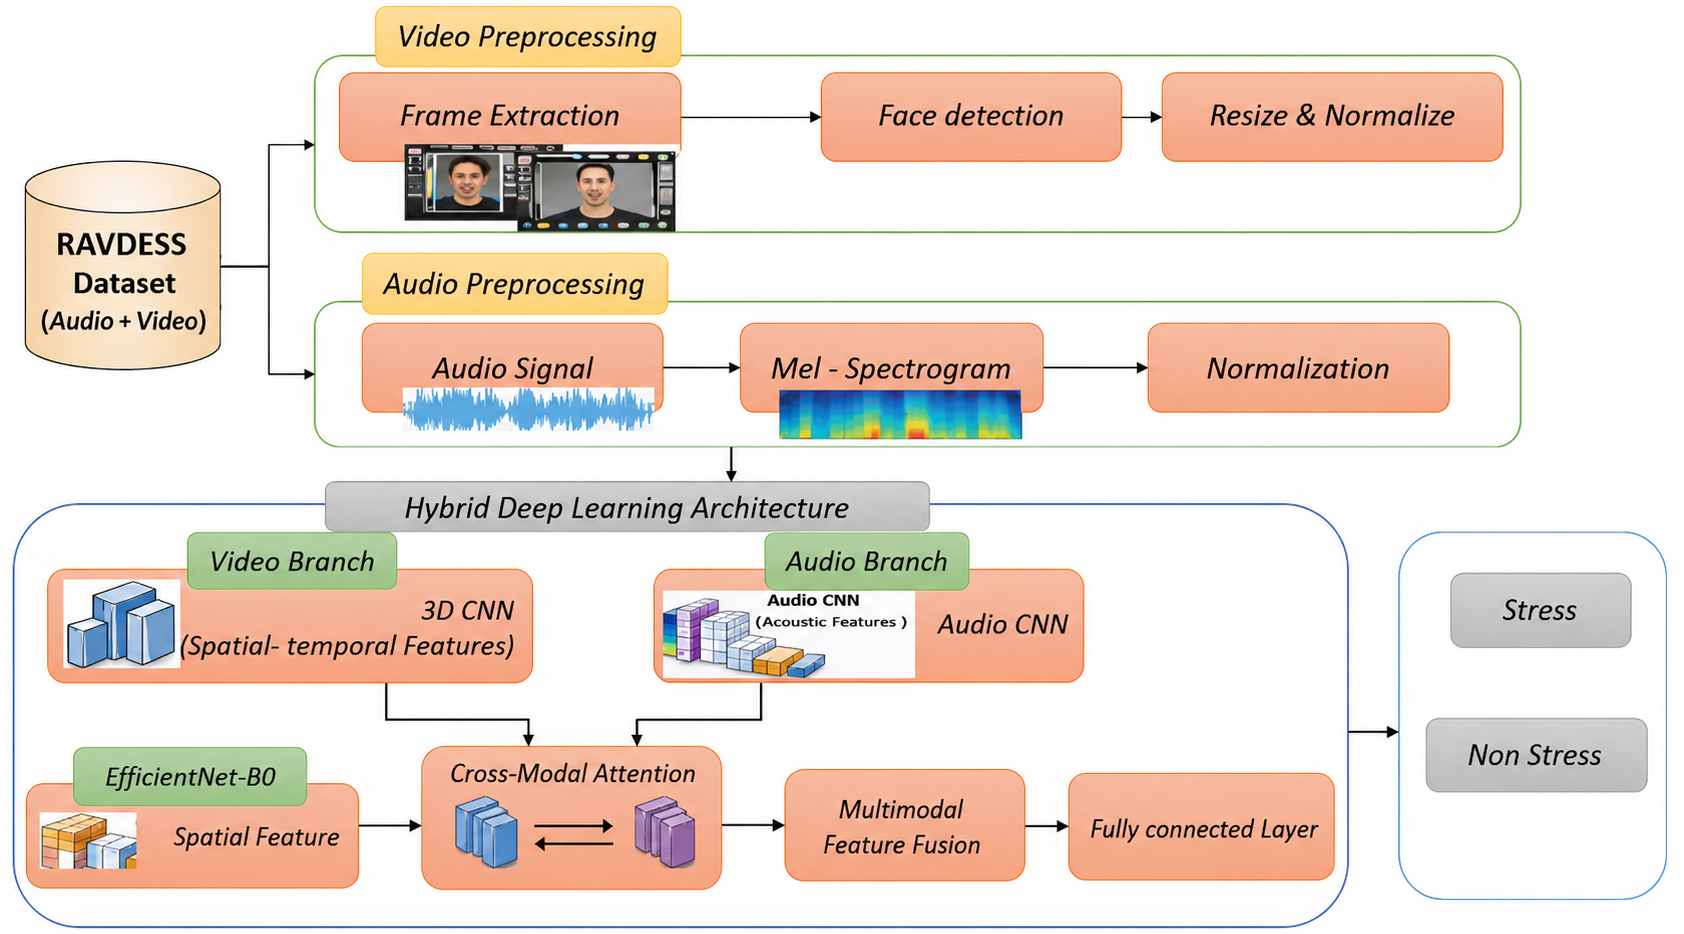
\includegraphics[width=0.75\textwidth]{pro.png}
\caption{Proposed Multimodal Stress Detection Framework}
\label{fig:sample}
\end{figure*}

\subsection{Dataset}

The publicly available RAVDESS dataset is used in this study. It contains audio–visual recordings of speeches with different emotional expressions performed by 24 professional actors (12 male and 12 female)~\cite{ref5}. Eight emotional states—neutral, calm, happy, sad, angry, fearful, disgusted, and surprised—are expressed by each actor. The recordings include high-quality video synchronized with speech signals. For stress detection, emotions like anger, fear, and sadness are categorized as stress-related, while calm and neutral are considered non-stress. Fixed-length 2-second clips were extracted with a 0.5-second sliding-window stride, yielding a balanced set of 1000 samples (500 stress, 500 non-stress). The structured nature of the dataset enables evaluation of calibration and uncertainty mechanisms.

\subsection{Preprocessing and Segmentation}

Video clips are converted into frame sequences, from which facial regions are detected, cropped, resized to a consistent resolution, and normalized. Each video is then split into fixed-length frame sequences so that the 3D-CNN can model temporal changes in facial expression. Speech signals are normalized, segmented into matching short intervals, and converted into Mel-spectrogram representations that capture the acoustic dynamics associated with stress.

\subsection{Feature Extraction Using Deep Learning}

Deep learning architectures automatically learn discriminative features from the visual and acoustic modalities. Throughout, $d$ denotes the common embedding dimension shared by all branches.

\begin{itemize}

\item \textbf{3D Convolutional Neural Network (3D-CNN)}

The 3D-CNN extracts spatio-temporal features from the facial video sequence, jointly modelling the spatial and temporal dimensions of convolution to learn dynamic patterns of facial expressions~\cite{ref7}. Its output is a short-term visual feature vector $f_s \in \mathbb{R}^{d}$.

\item \textbf{EfficientNet-B0}

High-level spatial features are extracted from each facial frame using EfficientNet-B0, which employs compound scaling to balance network depth, width, and input resolution for efficient feature learning with fewer parameters~\cite{ref6}. The per-frame embeddings are refined by a Transformer encoder, yielding a frame-level visual sequence $F_v \in \mathbb{R}^{L_v \times d}$ and a pooled visual vector $f_v \in \mathbb{R}^{d}$, where $L_v$ is the number of frames.

\item \textbf{Audio Branch}

In parallel, the acoustic branch encodes speech features into an audio sequence $F_a \in \mathbb{R}^{L_a \times d}$ and a pooled audio vector $f_a \in \mathbb{R}^{d}$, where $L_a$ is the number of audio frames.

\end{itemize}

\subsection{Multimodal Feature Fusion}

The speech and facial signals carry complementary information, so we combine them using cross-modal attention followed by feature concatenation.

Cross-attention lets one modality look at the most relevant parts of the other. We write $\mathrm{MHA}(Q,K,V)$ for multi-head attention (with query $Q$, key $K$, and value $V$) and $\mathrm{LN}(\cdot)$ for layer normalization, and define the operator $\mathrm{CA}(Q,K)=\mathrm{LN}(Q+\mathrm{MHA}(Q,K,K))$. Using the pooled vector of one modality as the query and the frame sequence of the other as key and value, we get an audio-aware visual vector $\tilde{v}$ and a visual-aware audio vector $\tilde{a}$:
\begin{equation}
\tilde{v} = \mathrm{CA}(f_v, F_a), \quad \tilde{a} = \mathrm{CA}(f_a, F_v).
\end{equation}

These attended vectors are concatenated with the short-term visual vector to form the fused representation $f = [\,f_s \oplus \tilde{v} \oplus \tilde{a}\,]$, where $\oplus$ denotes concatenation. This representation captures the facial and speech cues linked to stress. Such multimodal fusion is widely used in affective computing to make predictions more robust~\cite{ref2}.
\subsection{Model Training and Stress Classification}

The fused feature $f$ passes through fully connected layers that output a single number, the logit $\ell = \phi(f)$; a larger logit means the model leans towards \textit{Stress}. Instead of turning this logit into a probability directly, we first divide it by a temperature $T$, a simple step that makes the confidence scores more trustworthy (better calibrated). The stress probability is
\begin{equation}
p = \sigma(\ell / T),
\end{equation}

where $\sigma(\cdot)$ is the sigmoid. We choose the best temperature $T^{*}$ on the validation set so that the predicted probabilities match the true labels as closely as possible, i.e. by minimizing the negative log-likelihood (NLL) over the $N$ samples with labels $y_i \in \{0,1\}$ and logits $\ell_i$:
\begin{equation}
\begin{split}
T^{*} = \arg\min_{T>0} -\frac{1}{N}\sum_{i=1}^{N}\big[\, & y_i \log \sigma(\ell_i/T) \\
& + (1-y_i)\log\big(1-\sigma(\ell_i/T)\big) \big].
\end{split}
\end{equation}

This yields $T^{*}=3.0855$. The network is trained with backpropagation using binary cross-entropy on the logits, and we report the standard metrics: accuracy, precision, recall, F1-score, and Area Under the Curve (AUC).

\subsection{Uncertainty-Aware Prediction}

A single prediction does not tell us how sure the model is. To measure confidence we use Monte Carlo (MC) Dropout: we keep dropout switched on during testing and run the same input $M=20$ times, each run giving a slightly different probability $p_t = \sigma(\ell_t/T^{*})$. If the runs agree the model is confident; if they disagree it is uncertain. We summarise the runs by their mean $\bar{p}$ and variance:
\begin{equation}
\begin{aligned}
\bar{p} &= \frac{1}{M}\sum_{t=1}^{M} p_t, \\
\mathrm{Var} &= \frac{1}{M}\sum_{t=1}^{M} (p_t - \bar{p})^2.
\end{aligned}
\end{equation}

A larger variance means higher uncertainty. Uncertainty can also be measured with entropy. Using the binary entropy $H(p) = -[\,p\ln p + (1-p)\ln(1-p)\,]$, the total uncertainty is the entropy of the mean, $H(\bar{p})$, while the part caused by the model itself (epistemic uncertainty) is the mutual information $I$:
\begin{equation}
\begin{aligned}
H(\bar{p}) &= -[\,\bar{p}\ln\bar{p} + (1-\bar{p})\ln(1-\bar{p})\,], \\
I &= H(\bar{p}) - \frac{1}{M}\sum_{t=1}^{M} H(p_t).
\end{aligned}
\end{equation}

Finally, the model can choose not to answer when it is unsure. Let $u(x)$ be the uncertainty of a sample (its variance or entropy) and $\alpha \in [0,1]$ the fraction of samples we allow it to skip. Keeping only the most confident samples---those with $u(x) \le \eta_\alpha$, where $\eta_\alpha$ is the matching threshold---gives a coverage of $1-\alpha$. We check how well confidence matches accuracy using the Expected Calibration Error (ECE), computed over $B$ confidence bins $\mathcal{B}_b$:
\begin{equation}
\begin{gathered}
\hat{y}(x)\ \text{is predicted only if}\ u(x) \le \eta_\alpha, \\
\mathrm{ECE} = \sum_{b=1}^{B} \frac{|\mathcal{B}_b|}{N}\,\big|\mathrm{acc}(\mathcal{B}_b) - \mathrm{conf}(\mathcal{B}_b)\big|.
\end{gathered}
\end{equation}

A lower ECE means the model's confidence is more reliable.

\section{Results and Discussion}

This section provides a comprehensive analysis of \textbf{UA-HybridNet}, which combines uncertainty estimation and probability calibration with the Hybrid (3D-CNN + EfficientNet-B0 + Cross-Attention) architecture.

\subsection{Experimental Setup}
The 1000 clips were divided using a 70/15/15 stratified split (seed 42), giving 700 training, 150 validation, and 150 test samples with balanced classes. Partitioning was performed at the clip level by stratified random sampling, so clips from the same actor may span splits; the evaluation is thus not strictly subject-independent (see Limitations). All hyperparameters are listed in Table~\ref{tab:exp_config}.

\begin{table}[tb]
\centering
\caption{Experimental Configuration}
\label{tab:exp_config}
\footnotesize
\setlength{\tabcolsep}{3pt}
\renewcommand{\arraystretch}{1.1}
\begin{tabular}{llll}
\hline
\textbf{Parameter} & \textbf{Value} & \textbf{Parameter} & \textbf{Value} \\
\hline
Total samples      & 1000 (500/500) & Dropout rate       & 0.3 \\
Train/Val/Test     & 700/150/150    & MC Dropout ($T$)   & 20 \\
Split              & 70/15/15 strat.& TTA copies ($N$)   & 5 \\
Optimizer          & AdamW (wd $10^{-5}$) & Temperature ($T$) & 3.0855 \\
Learning rate      & $10^{-4}$      & Precision          & 16-bit mixed \\
Batch size         & 4 (eff.\ 16)   & Random seed        & 42 \\
LR schedule        & Cosine anneal. & Max epochs         & 100 (pat.\ 20) \\
\hline
\end{tabular}
\end{table}

\subsection{Performance Analysis}

\subsubsection{Overall Classification Performance}

A relative performance analysis of all explored architectures, including the baseline CNN–LSTM model, the cross-attention dual-stream model, the deterministic Hybrid architecture, and the suggested framework, is shown in Table~\ref{tab:all_arch_comparison}.

\begin{table}[tb]
\centering
\caption{Performance Comparison Across All Architectures}
\label{tab:all_arch_comparison}
\footnotesize
\resizebox{\columnwidth}{!}{%
\setlength{\tabcolsep}{1.7pt}
\renewcommand{\arraystretch}{1.3}
\begin{tabular}{lcccccc}
\hline
\textbf{Model} & \textbf{Acc.} & \textbf{Prec.} & \textbf{Recall} & \textbf{F1} & \textbf{AUC} & \textbf{Reliability} \\
\hline
Baseline (CNN-2D + LSTM)
  & \textbf{0.885} & \textbf{0.860} & 0.920 & \textbf{0.889} & \textbf{0.971} & No \\
Cross-Attention (Dual-Stream)
  & 0.790 & 0.790 & 0.790 & 0.790 & 0.890 & No \\
Hybrid (3D-CNN + EfficientNet-B0)
  & 0.850 & 0.802 & \textbf{0.930} & 0.861 & 0.940 & No \\
Hybrid + Uncertainty Modeling
  & 0.813 & 0.783 & 0.867 & 0.823 & 0.878 & \textbf{Yes} \\
\hline
\end{tabular}%
}
\end{table}

Even though the deterministic Hybrid model gives higher raw accuracy, UA-HybridNet prefers computed, uncertainity-aware predictions over point-estimate optimization. In healthcare stress monitoring areas of safety-critical applications, overconfidence and wrong estimates can have serious consequences. So as a result, reliability, compute quality and selective control of risk are more important than minor improvements in raw accuracy. The results show that UA-HybridNet significantly improve confidence arrangement and risk-aware decision making while maintaining competitive level classification performance. As the last two rows of Table~\ref{tab:all_arch_comparison} show, the deterministic Hybrid model attains higher raw accuracy but gives no calibrated confidence estimates, which are necessary in safety-critical applications for reliable deployment.

\subsubsection{Per-Class Performance}
For a balanced test set of 150 samples (75 stress and 75 non-stress) the per-class classification report is shown in Table~\ref{tab:perclass_pipelineD}. The results show that the stress class achieves higher recall (0.8667), indicating strong sensitivity in detecting stress, while the non-stress class achieves higher precision (0.8507); the macro and weighted averages remain balanced across precision, recall, and F1-score.
\begin{table}[tb]
\centering
\caption{Per-Class Classification Report for UA-HybridNet}
\label{tab:perclass_pipelineD}
\footnotesize
\setlength{\tabcolsep}{3pt}
\renewcommand{\arraystretch}{1.0}
\begin{tabular}{lcccc}
\hline
\textbf{Class} & \textbf{Precision} & \textbf{Recall} & \textbf{F1 Score} & \textbf{Support} \\
\hline
Stress     & 0.7831 & 0.8667 & 0.8228 & 75 \\
Non-Stress & 0.8507 & 0.7600 & 0.8028 & 75 \\
\textbf{Macro Avg}    & \textbf{0.8169} & \textbf{0.8133} & \textbf{0.8128} & \textbf{150} \\
\textbf{Weighted Avg} & \textbf{0.8169} & \textbf{0.8133} & \textbf{0.8128} & \textbf{150} \\
\hline
\end{tabular}
\end{table}

A wide perspective of classification results given by the confusion matrix is shown in Fig.~\ref{fig:pipd_confmat}. Out of the 150 test samples, 28 are incorrectly classified, and 122 are correctly classified.

\begin{figure}[tb]
\centering
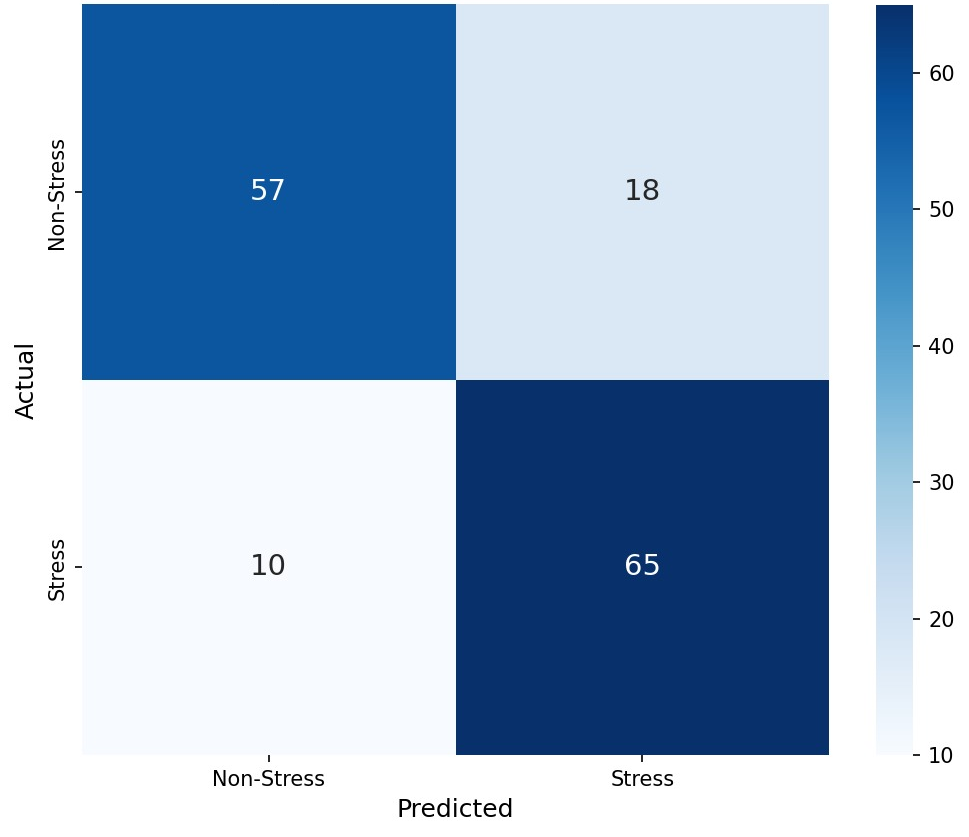
\includegraphics[width=0.9\linewidth]{confusion_matrix.png}
\caption{Confusion Matrix for UA-HybridNet.}
\label{fig:pipd_confmat}
\end{figure}

\subsubsection{Calibration Performance}

The crucial part of probability calibration is Temperature scaling. Calibration metrics are shown in Table~\ref{tab:calibration_metrics}, of both before and after scaling with a learning temperature parameter of $T = 3.0855$.
By reducing the Expected Calibration Error (ECE) by 60\% and Maximum Calibration Error (MCE) by 67\%, the quality of calibration is greatly improved by temperature scaling.

\begin{table}[tb]
\centering
\caption{Calibration Metrics Before and After Temperature Scaling}
\label{tab:calibration_metrics}
\footnotesize
\setlength{\tabcolsep}{2.5pt}
\renewcommand{\arraystretch}{1.0}
\begin{tabular}{lccc}
\hline
Metric & Before & After & Improvement \\
\hline
ECE & 0.1768 & \textbf{0.0710} & $\downarrow$ 59.8\% \\
MCE & 0.7651 & \textbf{0.2531} & $\downarrow$ 66.9\% \\
Brier Score & 0.1734 & \textbf{0.1450} & $\downarrow$ 16.4\% \\
NLL & 0.7172 & \textbf{0.3940} & $\downarrow$ 45.1\% \\
\hline
\end{tabular}
\end{table}

Figure~\ref{fig:tempscale} further shows this improvement using reliability diagrams of before and after calibration.

\begin{figure}[tb]
\centering
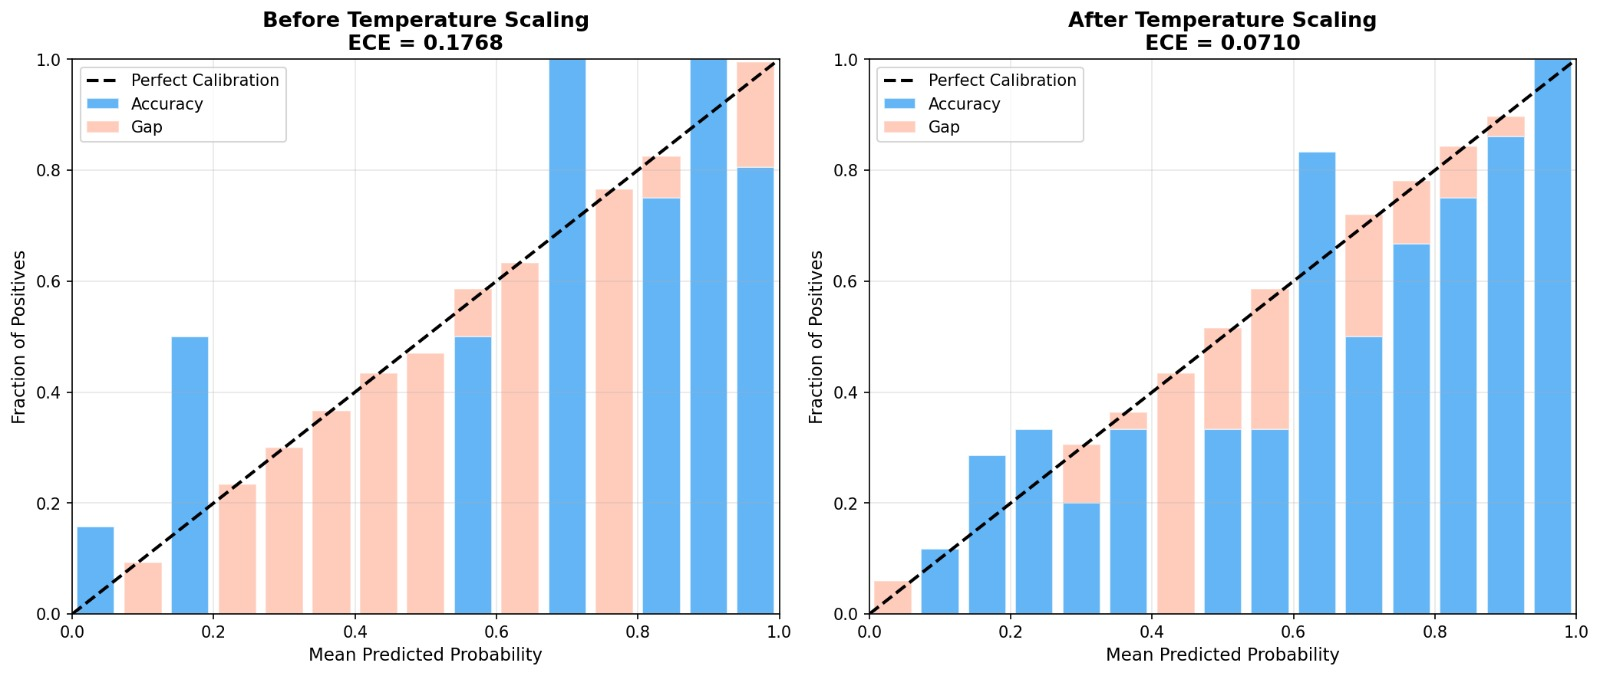
\includegraphics[width=\linewidth]{reliability_diagram.png}
\caption{Reliability diagrams before and after temperature scaling.}
\label{fig:tempscale}
\end{figure}

\subsubsection{Uncertainty Estimation Analysis}

Monte Carlo Dropout with $T = 20$ stochastic forward passes is used to estimate uncertainty. Key uncertainty measures, such as prediction variance, entropy, and the Uncertainty AUROC, are summarized in Table~\ref{tab:uncertainty_stats}.

\begin{table}[tb]
\centering
\caption{Uncertainty Estimation Statistics}
\label{tab:uncertainty_stats}
\footnotesize
\setlength{\tabcolsep}{3pt}
\renewcommand{\arraystretch}{1.0}
\begin{tabular}{lc}
\hline
Metric & Value \\
\hline
Mean Predictive Variance & 0.001564 \\
Mean Predictive Entropy & 0.1092 \\
Uncertainty AUROC & 0.6906 \\
Risk-Coverage AURC & 0.1015 \\
\hline
\end{tabular}
\end{table}
The misclassified samples generally show more predictive variance than correctly classified samples, which was confirmed by the uncertainty distribution shown in Fig.~\ref{fig:uncert}

\begin{figure}[tb]
\centering
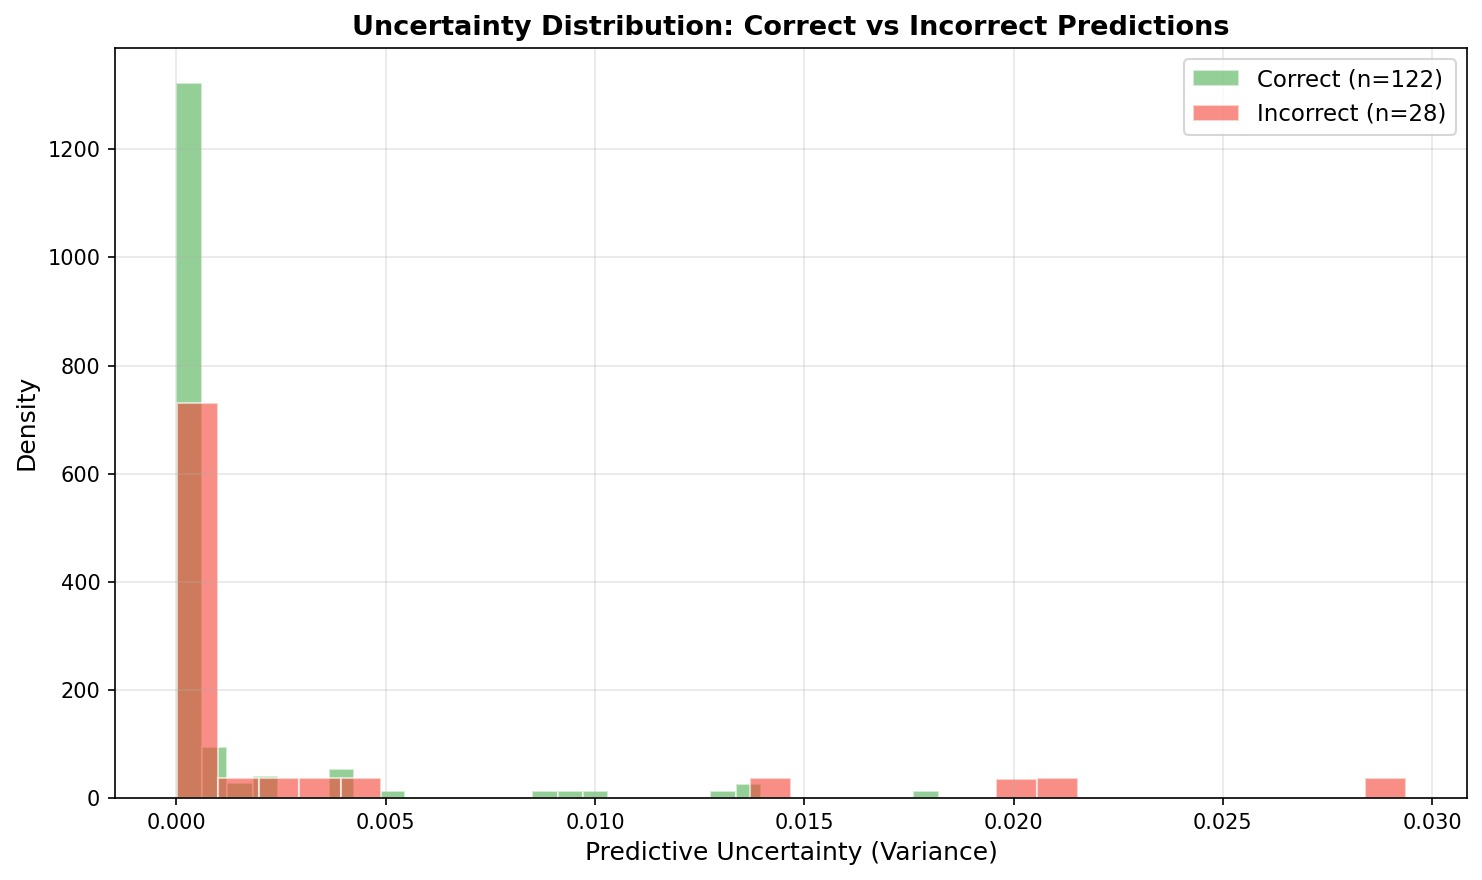
\includegraphics[width=0.9\linewidth]{uncertainty_distribution.png}
\caption{Predictive uncertainty distribution for correct and incorrect predictions.}
\label{fig:uncert}
\end{figure}
\subsubsection{Selective Prediction Performance}
Selective prediction experiments assess the effects of rejecting samples that may not be certain. Increasing the rejection rate progressively enhances classification performance, as Table~\ref{tab:selective_pred_full} demonstrates.

\begin{table}[tb]
\centering
\caption{Selective Prediction Performance at Different Rejection Levels}
\label{tab:selective_pred_full}
\footnotesize
\setlength{\tabcolsep}{1.5pt}
\renewcommand{\arraystretch}{1.0}
\begin{tabular}{lccccccc}
\hline
Rejection Rate & Kept & Rejected & Accuracy & Precision & Recall & F1 Score & AUC \\
\hline
0\% & 150 & 0  & 0.8133 & 0.7831 & 0.8667 & 0.8228 & 0.8782 \\
5\% & 143 & 7  & 0.8322 & 0.8077 & 0.8750 & 0.8400 & 0.8834 \\
10\% & 135 & 15 & 0.8296 & 0.8108 & 0.8696 & 0.8392 & 0.8887 \\
\textbf{20\%} & \textbf{120} & \textbf{30} & \textbf{0.8333} & \textbf{0.8088} & \textbf{0.8871} & \textbf{0.8462} & \textbf{0.8999} \\
\hline
\end{tabular}
\end{table}

Stress recall likewise rises from 0.8667 at full coverage to 0.8871 at a 20\% rejection rate, which is important for safety-sensitive monitoring where missed stress cases carry the higher cost. The risk-coverage curve in Fig.~\ref{fig:risk_curve} shows that rejecting high-uncertainty samples significantly reduces prediction error.
\begin{figure}[tb]
\centering
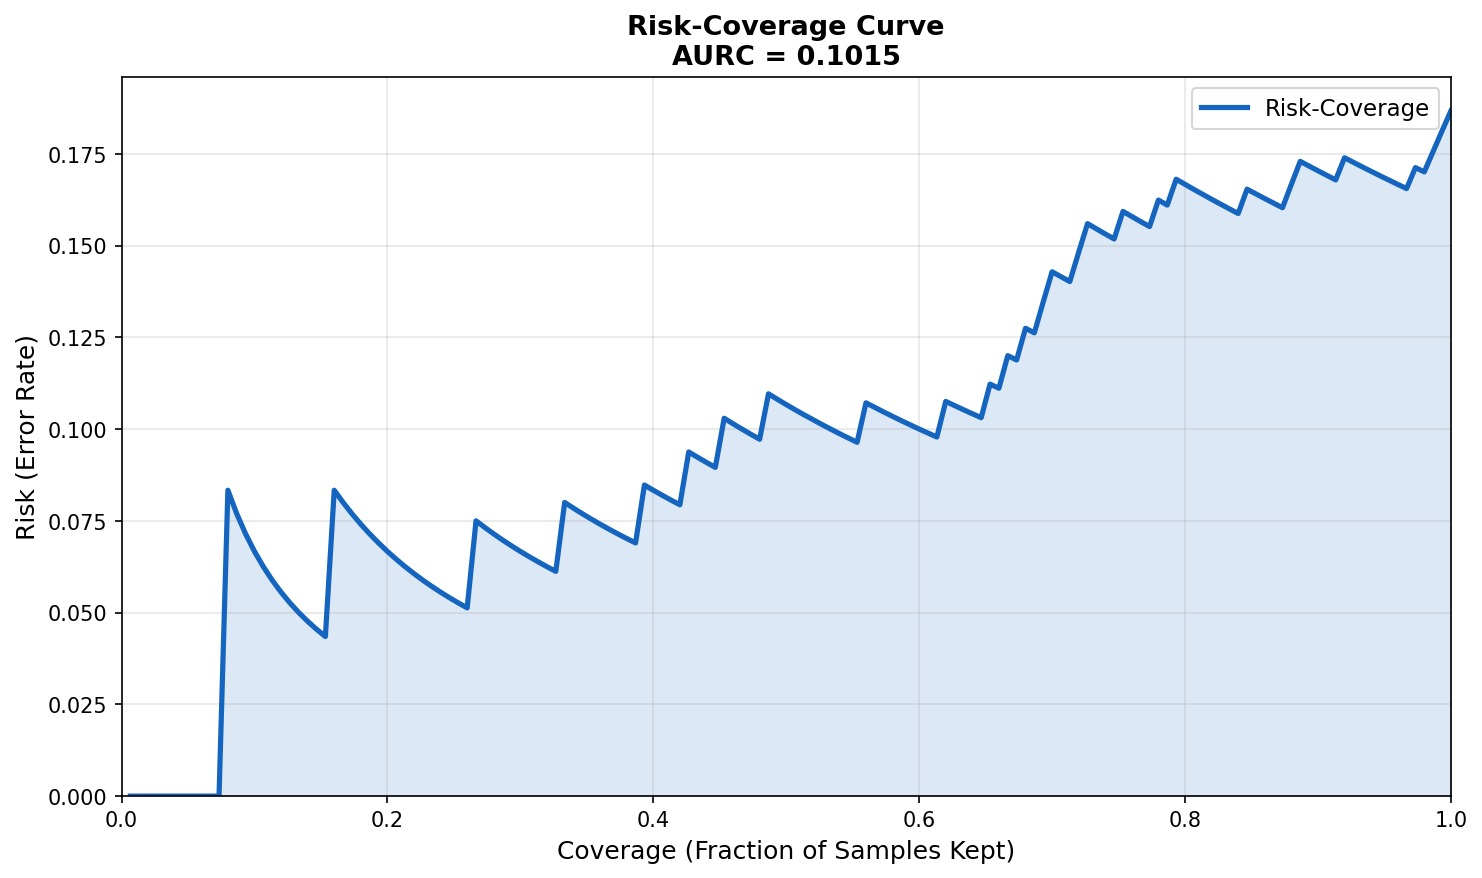
\includegraphics[width=0.9\linewidth]{risk_coverage.png}
\caption{Risk-Coverage Curve demonstrating uncertainty-aware error reduction.}
\label{fig:risk_curve}
\end{figure}

Overall, the results show that UA-HybridNet successfully involves uncertainty estimates and computation into deep multimodal feature learning, allowing reliable detection of stress with robustness and prediction with higher confidence.
The CNN-LSTM baseline gives deterministic predictions without confidence or quantifying the uncertainty of prediction, but achieves the highest possible classification of raw accuracy. By combining uncertainty estimation and probability calibration techniques, the suggested UA-HybridNet framework mainly focuses on reliability-aware modeling.
Through computed estimates of confidence and selective prediction of risk-awareness, this combination greatly increases the reliability of prediction with a small reduction in the point-estimate accuracy.
In application of safety-sensitive stress monitoring, where overconfident, incorrect predictions can lead to misleading decision, hence these characteristics are especially important.

\subsection{Limitations}
Although the proposed framework demonstrates encouraging performance, it still has several drawbacks. 
Firstly, the applicability to real-world settings may be impacted since the RAVDESS dataset includes performed emotional expressions rather than spontaneous real-world stress signals. 
Next, the size of the dataset is quite modest compared with other large-scale deep learning datasets. Larger multimodal datasets and real-time deployment situations will be the focus of future research. Because samples were split at the clip level, clips from the same actor may occur across splits, so results are not strictly subject-independent; a leave-actors-out protocol is planned as future work.

\subsection{Future Implications}

We are extending this work along four concrete directions. First, to directly justify the accuracy--reliability trade-off against the CNN-LSTM baseline, we will fit temperature scaling to the baseline's own logits and report its ECE/MCE alongside UA-HybridNet's (Table~\ref{tab:calibration_metrics}), rather than leaving the comparison one-sided. Second, since clips were split at the clip level rather than the actor level, we will re-evaluate all models under a leave-actors-out protocol to rule out speaker-identity leakage and confirm the reported accuracy holds for unseen speakers. Third, given the modest test set (n=150, 75/class), we will expand the evaluation set and run a paired McNemar's test on matched predictions to confirm the accuracy gap against the baseline is real; a preliminary 95\% Wilson interval already places UA-HybridNet's accuracy at [0.743, 0.868] against approximately [0.826, 0.928] for the baseline\footnote{Baseline count of 133/150 inferred from its reported 0.885 accuracy.}, motivating this as a priority. Finally, we will strengthen the uncertainty signal itself -- the current Uncertainty AUROC of 0.6906 is only a weak-to-moderate discriminator of misclassification -- by exploring deep ensembles and evidential deep learning as alternatives to MC Dropout, building on the gains already observed from selective prediction and uncertainty-based filtering (Table~\ref{tab:selective_pred_full}).

\section{Conclusion}


To detect facial stress, this research proposed an uncertainty-aware deep learning system which combines probabilistic calibration and uncertainty estimation with hybrid feature learning. The proposed model combines Monte-Carlo Dropout and temperature scaling with EfficientNet-B0 spatial feature extraction, 3D-CNN spatio-temporal encoding, and cross-modal attention fusion. A very strong classification performance is shown by the experimental findings on the RAVDESS dataset, with an accuracy of 0.8133 and an AUC of 0.8782. By reducing the negative log-likelihood by 45.1\% and the Expected Calibration Error (ECE) from 0.1768 to 0.0710, the calibration is greatly improved by temperature scaling and showed an increased agreement between actual accuracy and expected confidence.
Selective prediction further improved the system dependability: accuracy increased to 0.8333 and AUC to 0.8999 at a 20\% rejection rate. These results show that uncertainty estimation improves the overall reliability and successfully detects the incorrect predictions. 

Thus, the proposed model gives a useful and reliable foundation for applications requiring human-computer interaction, evaluation of workplace well-being, and stress monitoring in healthcare.

\begin{thebibliography}{99}

\bibitem{ref1}
S. Gedam and S. Paul,
"A review on mental stress detection using wearable sensors and machine learning techniques,"
IEEE Access, vol. 9, pp. 84045–84066, 2021.

\bibitem{ref2}
A. Mentis, D. Lee, and P. Roussos,
"Artificial intelligence applications for stress detection and mental health monitoring,"
Molecular Psychiatry, vol. 29, pp. 1503–1518, 2024.

\bibitem{ref3}
S. Hosseini, A. K. Bashivan, and N. Mehrabi,
"A multimodal sensor dataset for continuous stress detection of nurses in a hospital,"
Scientific Data, vol. 9, no. 255, 2022.

\bibitem{ref4}
T. Iqbal, M. Elahi, A. W. Malik, and S. M. N. Naqvi,
"Stress monitoring using wearable sensors: A pilot study and Stress-Predict dataset,"
Sensors, vol. 22, no. 21, 2022.

\bibitem{ref5}
S. R. Livingstone and F. A. Russo,
"The Ryerson Audio-Visual Database of Emotional Speech and Song (RAVDESS): A dynamic multimodal database of emotional expressions,"
PLoS ONE, vol. 13, no. 5, 2018.

\bibitem{ref6}
M. Tan and Q. V. Le,
"EfficientNet: Rethinking model scaling for convolutional neural networks,"
Proc. International Conference on Machine Learning (ICML), 2019.

\bibitem{ref7}
J. Carreira and A. Zisserman,
"Quo vadis, action recognition? A new model and the Kinetics dataset,"
Proc. IEEE Conference on Computer Vision and Pattern Recognition (CVPR), 2017.

\bibitem{ref8}
A. Vaswani et al.,
"Attention is all you need,"
Advances in Neural Information Processing Systems (NeurIPS), 2017.

\bibitem{ref9}
Y. Gal and Z. Ghahramani,
"Dropout as a Bayesian approximation: Representing model uncertainty in deep learning,"
Proc. International Conference on Machine Learning (ICML), 2016.

\bibitem{ref10}
C. Guo, G. Pleiss, Y. Sun, and K. Q. Weinberger,
"On calibration of modern neural networks,"
Proc. International Conference on Machine Learning (ICML), 2017.

\bibitem{ref11}
A. Kendall and Y. Gal,
"What uncertainties do we need in Bayesian deep learning for computer vision?"
Advances in Neural Information Processing Systems (NeurIPS), 2017.

\bibitem{ref12}
B. Lakshminarayanan, A. Pritzel, and C. Blundell,
"Simple and scalable predictive uncertainty estimation using deep ensembles,"
Advances in Neural Information Processing Systems (NeurIPS), 2017.

\bibitem{ref13}
Y. Geifman and R. El-Yaniv,
"Selective classification for deep neural networks,"
Advances in Neural Information Processing Systems (NeurIPS), 2017.

\bibitem{ref14}
D. Hendrycks and K. Gimpel,
"A baseline for detecting misclassified and out-of-distribution examples in neural networks,"
International Conference on Learning Representations (ICLR), 2017.

\bibitem{ref15}
M. Nag, J. Vijaya, and K. Mallikharjuna Rao,
"Enhanced Stress Prediction among Nurses in Their Work Environment Using Clustered Chameleon Swarm Algorithm,"
Proc. 3rd Cognitive Models and Artificial Intelligence Conference (AICCONF), IEEE Conference Proceedings, pp. 1--6, 2025.

\end{thebibliography}
\end{document}
